\chapter[~]{Методи кількісної оцінки ефективності та якості.  ослідження впливу коефіцієнтів важливості
  на результат прийняття рішень}

\textbf{Мета роботи} --- дослідити вплив зміни коефіцієнтів важливості на рішення, що приймаються,
визначити межі інтервалів зміни кожного коефіцієнту важливості, в яких рішення щодо найбільш
ефективної системи не змінюється.


\section{Короткі теоретичні відомості}

В даній лабораторній роботі необхідно дослідити варіанти систем, що розглядалися в першій
лабораторній роботі (ЛР), а саме потрібно визначити вплив значень окремих вагових коефіцієнтів на
результат в цілому. В першій ЛР було складено модель прийняття рішень щодо найбільш ефективної
системи, в якій серед інших параметрів фігурували коефіцієнти важливості показників.  Отже в даній
ЛР необхідно дослідити, як впливає зміна параметрів моделі прийняття рішень на результат.

Якщо при дослідженні моделі ставиться задача отримати результат не лише при певних конкретних
значеннях параметрів, а загалом на всій їх множині (тобто параметри не є фіксовані), то така задача
відноситься до задач проведення модельного експерименту. Для правильної організації модельного
експерименту необхідно володіти наступною інформацією про об’єкт дослідження чи аналізу.

\begin{enumerate}
\item Необхідно знати, до якого класу відноситься об’єкт, що моделюється: статичний (не змінюється в
  часі) чи динамічний (змінюється в часі), детермінований (не залежить від випадкових факторів) чи
  стохастичний (залежить від них).
\item Якщо об’єкт динамічний, то який режим його досліджується: стаціонарний (встановлений) чи
  нестаціонарний (перехідний процес), впродовж якого часу необхідно досліджувати об’єкт тощо.
\item Якщо об’єкт стохастичний, то який необхідно провести об’єм досліджень (кількість дослідів),
  щоб отримати достовірну інформацію та статистичні оцінки характеристик об’єкта.
\end{enumerate}

Об’єкти, що розглядалися в ЛР №1 вважаються статичними і детермінованими, тобто вважається, що їх
характеристики не залежать від часу та від випадкових факторів.

Тим не менш, оскільки параметри моделі прийняття рішень є варійованими, то необхідно визначити їх
множину, для якої проводити досліди. Очевидно, що досліджувати будь-яку систему у всіх режимах при
всіх умовах, тобто при всіх можливих співвідношеннях внутрішніх та зовнішніх параметрів досить
складно, витратно і в цьому немає практичного сенсу. Задача визначення складу множини варійованих
параметрів моделі називається пошуком плану експерименту.  Пошук плану експерименту виконується в
так званому факторному просторі.

\textbf{Факторний простір} --- це множина зовнішніх та внутрішніх параметрів моделі, значення яких
дослідник може контролювати в ході підготовки та проведення модельного експерименту.

Іншими словами, фактори --- це ті параметри, які є варійованими в моделі.  Фактори можуть мати
кількісний або якісний характер, виражати ступінь певної якості, змінюватись дискретно чи
неперервно. Тому значення факторів називають рівнями. Якщо при проведенні експерименту дослідник
може змінювати рівні факторів, експеримент називається активним, інакше – пасивним. Кожен фактор має
верхній та нижній рівні (межі змін), розташовані симетрично відносно певного нульового рівня. В
даній роботі експеримент є активним і факторами є значення коефіцієнтів важливості в моделі
прийняття рішень.

Як правило, план експерименту будується відносно певної однієї результуючої скалярної величини Y,
яка називається спостережуваною змінною. Якщо моделювання використовується як інструмент прийняття
рішень, то в ролі спостережуваної змінної виступає результуючий показник ефективності (як в нашому
випадку).

Якщо на об’єкт впливають випадкові фактори, то значення спостережуваної змінної $Y$ включає, крім
невипадкової функції факторів $f(x)$ (функції відгуку, що детерміновано залежить від значень
факторів), ще випадкову величину --- похибку експерименту $e(x)$:
\begin{equation}
  \label{eq:experimental_error}
  Y = f(x) + e(x)
\end{equation}

В такому випадку експерименти проводять в такому об’ємі, щоб статистичні оцінки випадкової величини
результату експерименту $Y$ задовольняли вимогам, що висуваються.

Існує дві постановки задачі планування експерименту:

\begin{enumerate}
\item \textbf{Стратегічне планування експерименту}. Обрати такий план експерименту, який би дав
  найбільш достовірне значення функції факторів $f(x)$ (та найбільш повну інформацію про результат)
  при фіксованому числі дослідів.
\item \textbf{Тактичне планування експерименту}. Обрати такий план, при якому функція $Y$ є
  достатньо точною в статистичному розумінні (статистичні оцінки задовольняють вимогам) при
  мінімальному об’ємі досліджень. Інакше, тактичне планування експериментів --- це сукупність
  методів встановлення необхідного об’єму повторних дослідів.
\end{enumerate}

Оскільки в нашому випадку об’єкт є детермінований, то повторних досліджень не вимагається. Отже
тактичне планування не є потрібним. Проте, необхідно врахувати підходи до стратегічного планування.

Отже, \textbf{метою стратегічного планування} є отримання максимального об’єму інформації про об’єкт
досліджень в кожному експерименті. Інакше, стратегічне планування дозволяє відповісти на питання,
при якому співвідношенні рівнів факторів може бути отримана найбільш повна та достовірна інформація
про поведінку об’єкта. При цьому вирішується дві основні задачі: \textbf{вибір складу факторів
  (ідентифікація факторів)} та \textbf{вибір рівнів факторів}.

Для даної ЛР склад факторів --- це набір з п’ятьох коефіцієнтів важливості.  Розглянемо детальніше
питання вибору рівнів факторів. Вибір рівнів факторів виконується із врахуванням двох протирічливих
вимог:
\begin{enumerate}
\item рівні кожного фактора мають перекривати (заповнювати) весь можливий діапазон його зміни;
\item загальна кількість рівній за всіма факторами не повинна призводити до надлишкового об’єму
  моделювання.
\end{enumerate}

Пошук компромісного рішення, яке задовольняє вказаним вимогам, є задачею стратегічного планування
експерименту.

\subsection{Способи побудови стратегічного плану}

\subsubsection{Повний факторний експеримент}

Експеримент, при якому реалізуються всі можливі співвідношення рівнів факторів, називається повним
факторним експериментом (ПФЕ). Загальна кількість різних комбінацій рівнів в ПФЕ для $k$ факторів буде
визначатися:

\begin{equation}
  \label{eq:pfe}
  N = l_1 \cdot l_2 \cdot l_3 \cdot \ldots \cdot l_i \cdot \ldots \cdot l_k
\end{equation}
\begin{itemize}[labelsep=*]
\item [де:] $l_i$ --- це число рівнів $k$-го фактору.
\end{itemize}

Якщо число рівнів для кожного фактору однакове і рівне $l$, то $N=l^k$.

\subsubsection{ Рандомізований план}

Передбачає вибір співвідношень рівнів для кожного досліду випадково. При цьому кількість
згенерованих комбінацій відповідає кількості дослідів, які необхідно провести

\subsubsection{Латинський план (латинський квадрат)}

Використовується в тому випадку, коли проводиться експеримент з одним первинним фактором (найбільш
важливим, вплив якого досліджується) та декількома вторинними (вплив яких не є предметом
досліджень). Зміст такого плану полягає в наступному. Якщо первинний фактор А має $l$ рівнів, то для
кожного вторинного фактору обирається також $l$ рівнів.

Вибір комбінацій рівнів виконується згідно спеціальної процедури. Наприклад, нехай крім первинного
фактору $А$, є два вторинні --- $В$ та $С$. Нехай кількість рівнів $l=4$. Тоді відповідний план
можна представити квадратною матрицею розміром $l \times l$ (тобто $4 \times 4$) відносно рівнів
фактору $А$.  При цьому матриця будується таким чином, щоб в кожному рядку та кожному стовбці даний
рівень фактору $А$ зустрічався лише один раз. (див \ref{t:latin_experiment})

\begin{table}[!ht]
\centering
\caption{Приклад латинського плану експерименту}
\label{t:latin_experiment}
\begin{tabular}{|c|c|c|c|c|}
\hline
\multirow{2}{*}{Значення  фактору В} & \multicolumn{4}{c|}{Значення фактору С} \\ \cline{2-5} 
 & C1 & C2 & C3 & C4 \\ \hline
B1 & A1 & A2 & A3 & A4 \\ \hline
B2 & A2 & A3 & A4 & A1 \\ \hline
B3 & A3 & A4 & A1 & A2 \\ \hline
B4 & A4 & A1 & A2 & A3 \\ \hline
\end{tabular}
\end{table}

В такому випадку замість $4^3 = 64$ досліди всього проводиться $4 \cdot 4=16$.

\subsubsection{Експеримент зі зміною факторів по одному}

В такому підході один з факторів приймає по-черзі всі $l$ рівнів, тоді як інші фактори залишаються
постійними. Такий план забезпечує дослідження впливу кожного фактору окремо. При цьому загальна
кількість дослідів:
\begin{equation}
  \label{eq:exp_one_by_one}
  N = l_1 + l_2 +l_3+ \ldots + l_k.
\end{equation}
Якщо всі фактори мають однакову кількість рівнів $l$, то $N = k \cdot l$. Для 3-х факторів по 4
рівні це буде 12 дослідів. Для оцінки об’єктів, що досліджуються в ЛР №1 такий план буде вимагати
максимум $21+21+21+21+21 = 105$ дослідів (замість кількості порядку 100000).

\subsubsection{Дробний факторний експеримент}

В такому випадку для кожного фактору беруться лише два рівня, що відповідають граничним значенням,
що може приймати фактор, --- верхнє та нижнє. Загальна кількість дослідів в такому випадку $N = 2^k$ , де
$k$ – кількість факторів.

\subsection{Обраний метод експеримету}

Отже, з метою спрощення досліджень та скорочення кількості дослідів в якості плану для експерименту
\textbf{в даній роботі обрано варіант експерименту зі зміною факторів по одному}. Особливість підходу, що
використовується в даній ЛР полягає в тому, що при дослідженні кожного з 5-ти параметрів, інші
будуть автоматично корегуватися відповідно вимог нормування.


Зокрема в програмі для даної ЛР реалізовано автокорекцію, що при зменшенні певного коефіцієнту
важливості на величину Δ (за модулем), інші автоматично зростають кожен на Δ/4 (за модулем).

При збільшенні певного коефіцієнту важливості на величину $\Delta$ (за модулем), виконуються наступні
правила:

\begin{enumerate}
\item Інші коефіцієнти автоматично зменшуються за модулем кожен на $\Delta / n$ (де n–кількість
  ненульових коефіцієнтів), якщо при цьому вони не змінюють знак. Інакше діє правило 2.
\item Зменшення відбувається на величину, на яку найближчий до 0 коефіцієнт відрізняється від 0, а
  потім --- відповідно до правила 1.
\end{enumerate}

\section{Порядок виконання роботи}

\subsection{Вихідні дані}

Навести вихідні дані про технічний об’єкт (чи систему) з ЛР №1 (\ref{t:source_data}). Бажано
також навести знімок екрану з результатами розрахунку на ЕОМ з ЛР №1.

\begin{table}[!ht]
\centering
\caption{Вихідні дані для оцінки ефективності}
\label{t:source_data_2}
\begin{tabular}{|C{2.4cm}|C{2.0cm}|C{2.6cm}|C{2.2cm}|C{2.1cm}|C{2.6cm}|}
\hline
Варіанти SSD & Обсяг, GB & Швидкість зчитування, Mb/s & Швидкість запису, Mb/s & Ціна, тис. грн. & Час наробки на відмову, млн годин \\ \hline
Kingston SSDNow KC400 & $128$ & $550$  & $450$ & $0.1$ & $1$ \\ \hline
Kingston HyperX Fury & $120$ & $ 500$ & $500$ & $0.5$ & $1$ \\ \hline
Kingston SSDNow V300 & $120$ & $ 450$ &  $450$& $0.4$ & $1$ \\ \hline
Коефіцієнт важливості $a_i$ ($b_j$) & $0.2$ & $0.3$ & $0.3$ & $-0.15$  & $0.05$ \\ \hline
\end{tabular}
\end{table}

\subsection{Визначення інтервалів}

За допомогою програми було визначено інтервали змін (максимальне та мінімальне можливе значення)
кожного з вагових коефіцієнтів окремо, в межах яких (включаючи межі) рішення щодо найбільш
ефективної системи не змінюється у порівнянні з даними першої лабораторної роботи (даними по
замовченню), тобто є таким самим, як в першій роботі. Для цього було виконано 14 загальних дослідів
(по 2 для кожного параметру):

\begin{enumerate}
\item Визначено мінімальне значення $a_{1 \text{ min}}$.
\item Визначено максимальне значення $a_{1 \text{ max}}$.
\item Визначено мінімальне значення $a_{2 \text{ min}}$.
\item Визначено максимальне значення $a_{2 \text{ max}}$.
\item Визначено мінімальне значення $a_{3 \text{ min}}$.
\item Визначено максимальне значення $a_{3 \text{ max}}$.
\item Визначено мінімальне значення $a_{4 \text{ min}}$.
\item Визначено максимальне значення $a_{4 \text{ max}}$.
\item Визначено мінімальне значення $a_{5 \text{ min}}$.
\item Визначено максимальне значення $a_{5 \text{ max}}$.
\end{enumerate}

\begin{figure}[H]
  \centering
  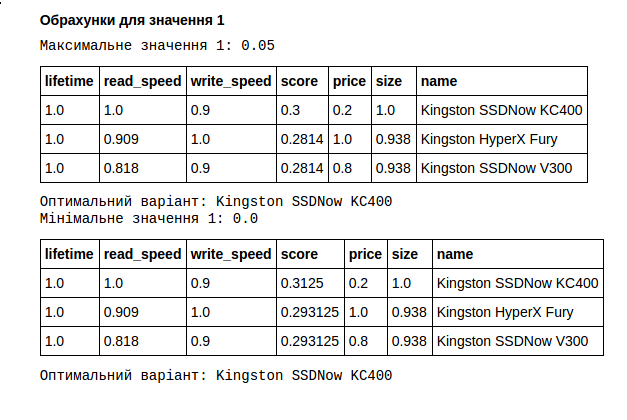
\includegraphics[width=.9\linewidth]{images/lab2/min_max_1.png}
  \label{f:min_max_a_1} 
  \caption{Мінімальне та максимальне значення $a_{1 \text{ min}}$, $a_{1 \text{ max}}$.}
\end{figure}
\begin{figure}[H]
  \centering
  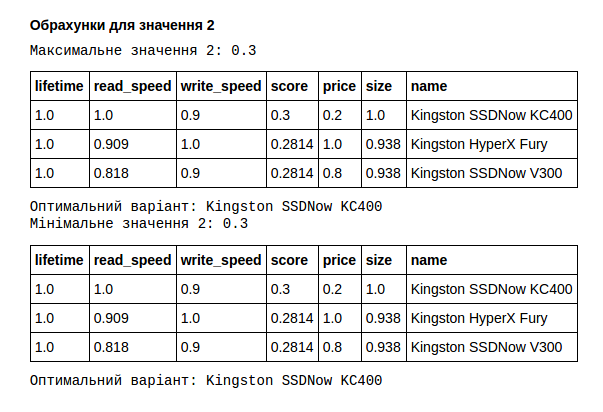
\includegraphics[width=.9\linewidth]{images/lab2/min_max_2.png}
  \label{f:min_max_a_2} 
  \caption{Мінімальне та максимальне значення $a_{2 \text{ min}}$, $a_{2 \text{ max}}$.}
\end{figure}
\begin{figure}[H]
  \centering
  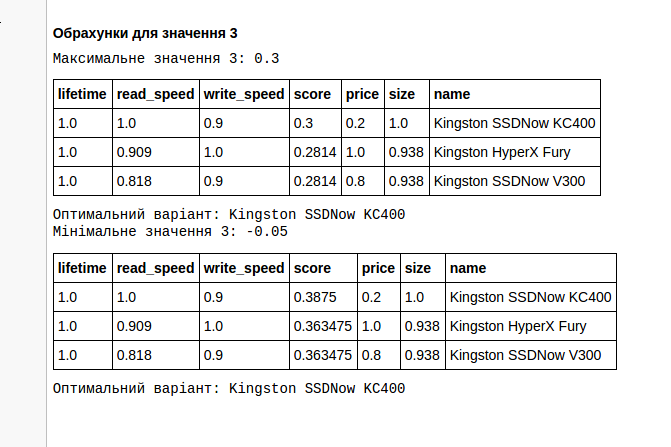
\includegraphics[width=.9\linewidth]{images/lab2/min_max_3.png}
  \label{f:min_max_a_3} 
  \caption{Мінімальне та максимальне значення $a_{3 \text{ min}}$, $a_{3 \text{ max}}$.}
\end{figure}
\begin{figure}[H]
  \centering
  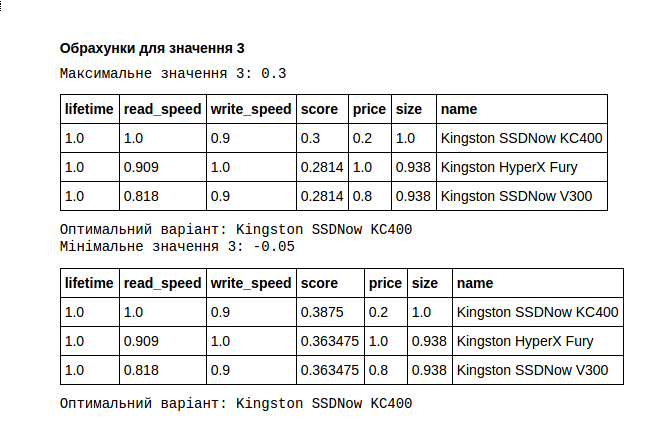
\includegraphics[width=.9\linewidth]{images/lab2/min_max_4.png}
  \label{f:min_max_a_4} 
  \caption{Мінімальне та максимальне значення $a_{4 \text{ min}}$, $a_{4 \text{ max}}$.}
\end{figure}
\begin{figure}[H]
  \centering
  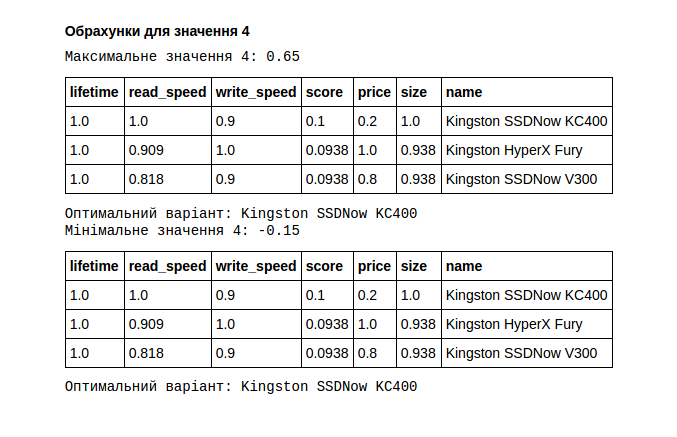
\includegraphics[width=.9\linewidth]{images/lab2/min_max_5.png}
  \label{f:min_max_a_5} 
  \caption{Мінімальне та максимальне значення $a_{5 \text{ min}}$, $a_{5 \text{ max}}$.}
\end{figure}

\newpage

\section*{Висновок}
У ході виконання лабораторної роботи було визначено інтервали змін (максимальне та мінімальне
можливе значення) кожного з вагових коефіцієнтів окремо, в межах яких (включаючи межі) рішення щодо
найбільш ефективної системи не змінюється у порівнянні з даними першої лабораторної роботи (даними
по замовченню), тобто є таким самим, як в першій роботі. Для цього було виконано 14 загальних
дослідів; по 2 для кожного параметру із 5 параметрів; по 5 мінімальних
($a_{1 \text{ min}} \ldots a_{5 \text{ min}}$) та 5 максимальних значень
($a_{1 \text{ max}} \ldots a_{5 \text{ max}}$). Графічно зображено інтервали в яких рішення щодо
найбільш ефективної системи не змінне.

Визначення цих інтервалів було здійснено за допомогою спеціального програмного середовища Jupyter.
